

\tikzset{every picture/.style={line width=0.75pt}} %set default line width to 0.75pt        

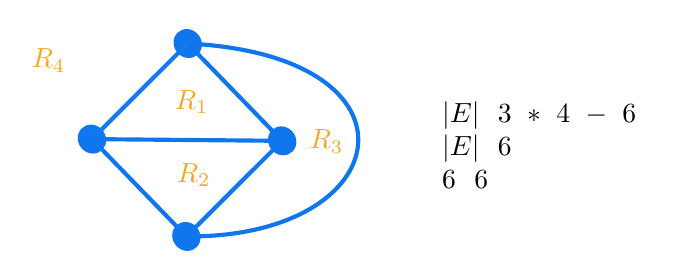
\begin{tikzpicture}[x=0.75pt,y=0.75pt,yscale=-1,xscale=1]
%uncomment if require: \path (0,129); %set diagram left start at 0, and has height of 129

%Shape: Ellipse [id:dp8824645259000807] 
\draw  [draw opacity=0][fill={rgb, 255:red, 15; green, 118; blue, 237 }  ,fill opacity=1 ] (83.4,5.3) .. controls (87.18,5.47) and (90.33,8.72) .. (90.45,12.57) .. controls (90.56,16.42) and (87.59,19.4) .. (83.82,19.23) .. controls (80.04,19.07) and (76.89,15.81) .. (76.77,11.96) .. controls (76.66,8.12) and (79.63,5.13) .. (83.4,5.3) -- cycle ;
%Shape: Ellipse [id:dp19463839491212043] 
\draw  [draw opacity=0][fill={rgb, 255:red, 15; green, 118; blue, 237 }  ,fill opacity=1 ] (37.25,51.36) .. controls (41.03,51.52) and (44.18,54.78) .. (44.29,58.63) .. controls (44.41,62.47) and (41.44,65.45) .. (37.67,65.29) .. controls (33.89,65.12) and (30.74,61.87) .. (30.62,58.02) .. controls (30.51,54.17) and (33.48,51.19) .. (37.25,51.36) -- cycle ;
%Straight Lines [id:da14445363951451218] 
\draw [color={rgb, 255:red, 16; green, 121; blue, 243 }  ,draw opacity=1 ][fill={rgb, 255:red, 0; green, 0; blue, 0 }  ,fill opacity=1 ][line width=1.5]    (83.61,12.27) -- (37.46,58.32) ;
%Shape: Ellipse [id:dp008236776664483747] 
\draw  [draw opacity=0][fill={rgb, 255:red, 15; green, 118; blue, 237 }  ,fill opacity=1 ] (128.91,52.18) .. controls (132.68,52.35) and (135.84,55.61) .. (135.95,59.45) .. controls (136.06,63.3) and (133.1,66.28) .. (129.32,66.11) .. controls (125.55,65.95) and (122.39,62.69) .. (122.28,58.85) .. controls (122.16,55) and (125.13,52.02) .. (128.91,52.18) -- cycle ;
%Shape: Ellipse [id:dp7929686215334855] 
\draw  [draw opacity=0][fill={rgb, 255:red, 15; green, 118; blue, 237 }  ,fill opacity=1 ] (82.76,98.24) .. controls (86.53,98.41) and (89.68,101.66) .. (89.8,105.51) .. controls (89.91,109.35) and (86.94,112.34) .. (83.17,112.17) .. controls (79.39,112) and (76.24,108.75) .. (76.13,104.9) .. controls (76.01,101.05) and (78.98,98.07) .. (82.76,98.24) -- cycle ;
%Straight Lines [id:da24639820678501922] 
\draw [color={rgb, 255:red, 15; green, 118; blue, 237 }  ,draw opacity=1 ][fill={rgb, 255:red, 0; green, 0; blue, 0 }  ,fill opacity=1 ][line width=1.5]    (129.11,59.15) -- (82.96,105.2) ;
%Straight Lines [id:da9492046865987103] 
\draw [color={rgb, 255:red, 15; green, 118; blue, 237 }  ,draw opacity=1 ][fill={rgb, 255:red, 0; green, 0; blue, 0 }  ,fill opacity=1 ][line width=1.5]    (83.61,12.27) -- (129.11,59.15) ;
%Straight Lines [id:da1986454721607971] 
\draw [color={rgb, 255:red, 15; green, 118; blue, 237 }  ,draw opacity=1 ][fill={rgb, 255:red, 0; green, 0; blue, 0 }  ,fill opacity=1 ][line width=1.5]    (37.46,58.32) -- (82.96,105.2) ;
%Straight Lines [id:da17378448524728318] 
\draw [color={rgb, 255:red, 15; green, 118; blue, 237 }  ,draw opacity=1 ][fill={rgb, 255:red, 0; green, 0; blue, 0 }  ,fill opacity=1 ][line width=1.5]    (129.11,59.15) -- (37.46,58.32) ;
%Curve Lines [id:da13127401435563257] 
\draw [color={rgb, 255:red, 15; green, 118; blue, 237 }  ,draw opacity=1 ][line width=1.5]    (83.61,12.27) .. controls (201.11,18.06) and (185.11,106.06) .. (82.96,105.2) ;

% Text Node
\draw (7,13.4) node [anchor=north west][inner sep=0.75pt]  [color={rgb, 255:red, 245; green, 166; blue, 35 }  ,opacity=1 ]  {$R_{4}$};
% Text Node
\draw (77,68.4) node [anchor=north west][inner sep=0.75pt]  [color={rgb, 255:red, 245; green, 166; blue, 35 }  ,opacity=1 ]  {$R_{2}$};
% Text Node
\draw (141,52.4) node [anchor=north west][inner sep=0.75pt]  [color={rgb, 255:red, 245; green, 166; blue, 35 }  ,opacity=1 ]  {$R_{3}$};
% Text Node
\draw (76,33.4) node [anchor=north west][inner sep=0.75pt]  [color={rgb, 255:red, 245; green, 166; blue, 35 }  ,opacity=1 ]  {$R_{1}$};
% Text Node
\draw (198,37.4) node [anchor=north west][inner sep=0.75pt]  [color={rgb, 255:red, 0; green, 0; blue, 0 }  ,opacity=1 ]  {$ \begin{array}{l}
|E|\ \leqslant \ 3\ *\ 4\ -\ 6\\
|E|\ \leqslant \ 6\\
6\ \leqslant \ 6\\
\end{array}$};


\end{tikzpicture}